
%(BEGIN_QUESTION)
% Copyright 2010, Tony R. Kuphaldt, released under the Creative Commons Attribution License (v 1.0)
% This means you may do almost anything with this work of mine, so long as you give me proper credit

Determine the value of the specified {\it integral} for this function:

$$\includegraphics[width=15.5cm]{i04370x01.eps}$$

$$\int_{-3}^{+4} f(x) \> dx$$

\vskip 20pt \vbox{\hrule \hbox{\strut \vrule{} {\bf Suggestions for Socratic discussion} \vrule} \hrule}

\begin{itemize}
\item{} A helpful hint when evaluating integrals is to determine the {\it sign} of the terms within the integrand over the specified interval.  Here, where the interval begins at $x=-3$ and continues to $x=+4$, what is the mathematical sign of $dx$?  Over this same interval, what is the mathematical sign of $f(x)$?
\item{} What is most important when solving problems such as this is to be able to explain {\it why} (not just {\it how}) to arrive at the correct value.  Try explaining the process of integration in your own words, as it applies to this particular problem.
\item{} Identify a practical, real-life example this graph might apply to.  Identify what the horizontal axis would represent, and what the vertical axis would represent, complete with units of measurement.
\end{itemize}

\underbar{file i04370}
%(END_QUESTION)





%(BEGIN_ANSWER)

-9

%(END_ANSWER)





%(BEGIN_NOTES)

Since the interval is specified as beginning at -3 and ending at +4, the direction of integration is left-to-right, and therefore each $dx$ differential will be positive in value.  This means any $y$ value below the zero line will yield a negative integrand (a negative times a positivei).





\vfil \eject

\noindent
{\bf Summary Quiz:}

Determine the value of the specified {\it integral} for this function:

$$\includegraphics[width=15.5cm]{i04370x02.eps}$$

$$\int_{-5}^{0} f(x) \> dx$$

\vskip 10pt

0 \hskip 40pt $-5$ \hskip 40pt $-1$  \hskip 40pt +11  \hskip 40pt +13  \hskip 40pt $-12$ \hskip 40pt +12



\vfil \eject

\noindent
{\bf Summary Quiz:}

Determine the value of the specified {\it integral} for this function:

$$\includegraphics[width=15.5cm]{i04370x02.eps}$$

$$\int_{-2}^{+5} f(x) \> dx$$

\vskip 10pt

+7 \hskip 40pt +6 \hskip 40pt 0  \hskip 40pt -2  \hskip 40pt +13  \hskip 40pt -7 \hskip 40pt +5


%INDEX% Mathematics, calculus: integral (approximating integral values between points on graph)

%(END_NOTES)


